\documentclass[handout,hyperref={colorlinks=true}]{beamer}
\usepackage[utf8]{inputenc}
\usepackage[T1]{fontenc}
\usepackage[finnish]{babel}
\usepackage{amsmath}
%\usepackage{amsfonts}
\usepackage{amssymb}
\usepackage{tikz}
\usepackage{framed}
\usepackage{alltt}
\usepackage{fancyvrb}
\usepackage{multirow}
\usepackage{mathtools}
\usepackage{multicol}
\usetikzlibrary{matrix,arrows,decorations.pathmorphing}
\usetikzlibrary{fadings,patterns,arrows}
%\pgfmathsetmacro{\inf}{-2}
%\pgfmathsetmacro{\sup}{2}
\tikzstyle{MyPlotStyle}=[domain=\inf:\sup,samples=100,smooth]
\usepgflibrary{arrows}
\newcounter{harkka}
\newtheorem{lause}{Lause}
\newtheorem*{huom}{Huomautus}
\newcounter{laskuri}
\newtheorem{trma}{Teoreema}[laskuri]
\newtheorem{prop}[trma]{Propositio}
\theoremstyle{remark}
\newtheorem{harj}{Harjoitus}[section]
\newtheorem*{esim}{Esimerkki}
\newtheorem*{ratk}{Ratkaisuehdotus}
\newtheorem*{extra}{Lisätieto}

\newcommand{\numeroi}{\stepcounter{harkka}\arabic{harkka}}
\newcommand{\vaihto}{\\ \vspace{10pt}}
\newcommand{\R}{\mathbb{R}\,}
\newcommand{\abs}[1]{\left|#1\right|}
\newcommand{\va}{\bar{a}}
\newcommand{\vb}{\bar{b}}
\newcommand{\vw}{\bar{w}}
\newcommand{\vv}{\bar{v}}
%\renewcommand*\env@matrix[1][*\c@MaxMatrixCols c]{%
%  \hskip -\arraycolsep
%  \let\@ifnextchar\new@ifnextchar
%  \array{#1}}
%\makeatother
%\newcommand{\abs}[1]{\left|#1\right|}
\newcommand{\BibTeX}{BibTeX}
%\newcommand{\bino}[2]{(x-#1)^{#2}}
\newcommand{\bino}[3]{\binom{#1}{#3}{#2}^{#3}(1-#2)^{#1-#3}}
\setbeamertemplate{theorems}[numbered]
\title{\LaTeX}
%Matriisien säätö:

\makeatletter
\renewcommand*\env@matrix[1][*\c@MaxMatrixCols c]{%
    \hskip -\arraycolsep
    \let\@ifnextchar\new@ifnextchar
\array{#1}}
\makeatother
\begin{document}
\setcounter{section}{2}
\begin{frame}
    \titlepage
\end{frame}
\begin{frame}
    \tableofcontents
\end{frame}
\section{3. kerta}
\subsection{Kuvat}
\subsubsection{Kuvien liittäminen}
\begin{frame}[fragile]
    \frametitle{Kuvien liittäminen}
    Kuvien liittämistä varten täytyy ottaa käyttöön \verb-graphicx--paketti. 
    \vaihto
    PDFLaTeXia käytettäessä sallitut kuvaformaatit ovat \verb-.pdf-, \verb-.jpg- ja \verb-.png-. 
    \vaihto
    Jos liitettävä kuva on samassa kansiossa muiden tiedostojen kanssa, kuvan liittäminen tapahtuu komennolla
    \begin{framed}
        \centering
        \verb-\includegraphics[asetukset]{kuvatiedoston_nimi}-. 
    \end{framed}
    Tiedostopäätettä ei ole tarpeen kirjoittaa, jos tiedoston nimi ei sisällä välejä.
    \vaihto
    Valinnaisella argumentilla voidaan skaalata, kiertää ja rajata liitettävää kuvaa. 
\end{frame}
\begin{frame}[fragile]
    \frametitle{Kuvien liittäminen}
    Työkansioon tallennetun kuvan \verb-smile.jpeg- saisi näkyviin koodilla
    \begin{scriptsize}
        \begin{Verbatim}[frame=single]
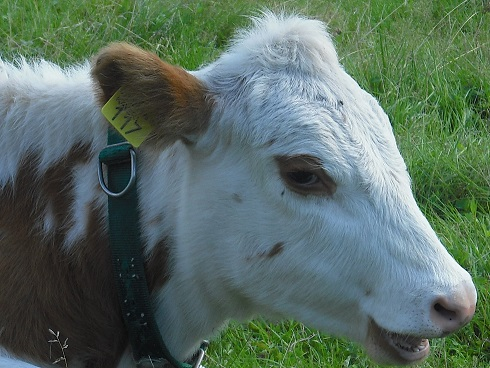
\includegraphics{smile}
        \end{Verbatim}
    \end{scriptsize}
    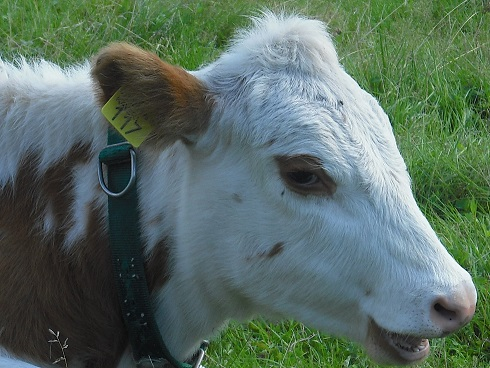
\includegraphics{smile}
\end{frame}
\begin{frame}[fragile]
    \frametitle{Kuvan skaalaus}
    Kuva on aivan liian suuri, joten sitä on syytä skaalata:
    \begin{scriptsize}
        \begin{Verbatim}[frame=single]
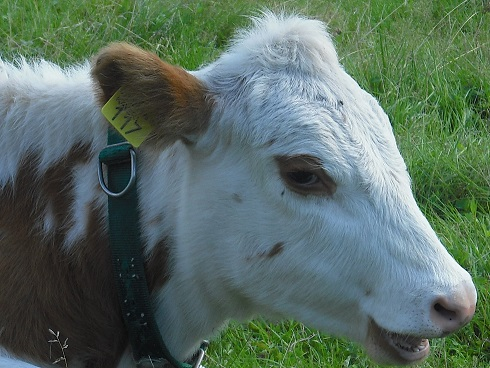
\includegraphics[scale=0.4]{smile}
        \end{Verbatim}
    \end{scriptsize}
    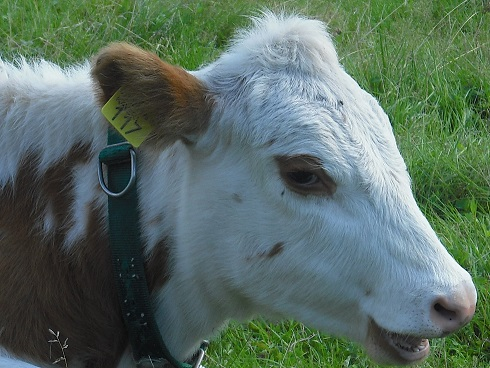
\includegraphics[scale=0.4]{smile}

\end{frame}
\begin{frame}[fragile]
    \frametitle{Kuvan skaalaus}
    Skaalaus onnistuu myös määrittelemällä kuvan leveys tai korkeus:
    \begin{scriptsize}
        \begin{Verbatim}[frame=single]
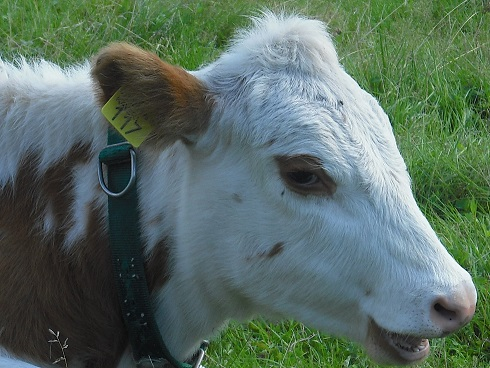
\includegraphics[width = 4cm]{smile}
        \end{Verbatim}
        \begin{Verbatim}[frame=single]
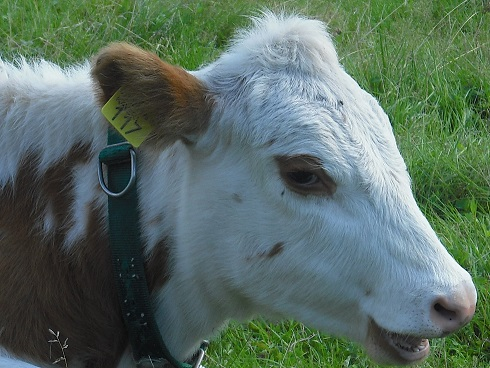
\includegraphics[height=4cm]{smile}
        \end{Verbatim}
    \end{scriptsize}
    \begin{minipage}{5cm}
        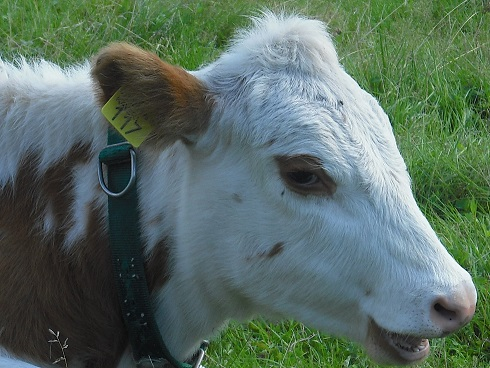
\includegraphics[width = 4cm]{smile}
    \end{minipage}
    \begin{minipage}{5cm}
        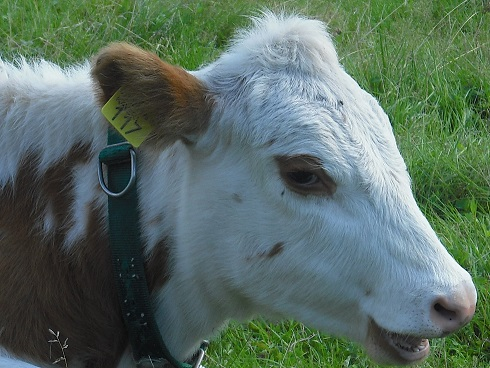
\includegraphics[height=4cm]{smile}
    \end{minipage}
\end{frame}
\begin{frame}[fragile]
    \frametitle{Kuvan kierto}
    Kuvaa voi kiertää antamalla valinnaiseksi argumentiksi kiertokulman asteina.

    \begin{scriptsize}
        \begin{Verbatim}[frame=single]
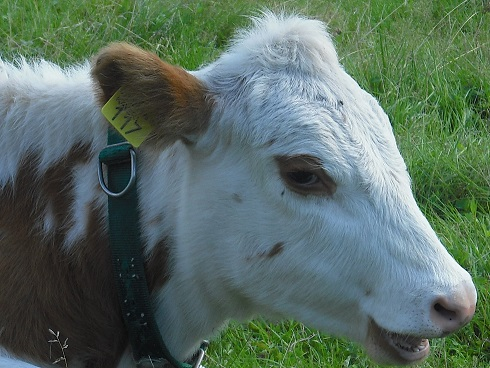
\includegraphics[width=4cm,angle=90]{smile}
        \end{Verbatim}
        \begin{Verbatim}[frame=single]
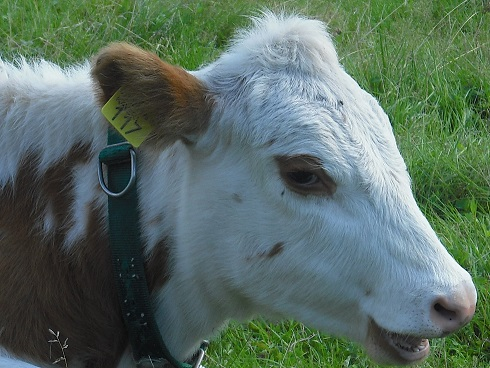
\includegraphics[height=4cm,angle=180]{smile}
        \end{Verbatim}
    \end{scriptsize}
    \begin{minipage}{3cm}
        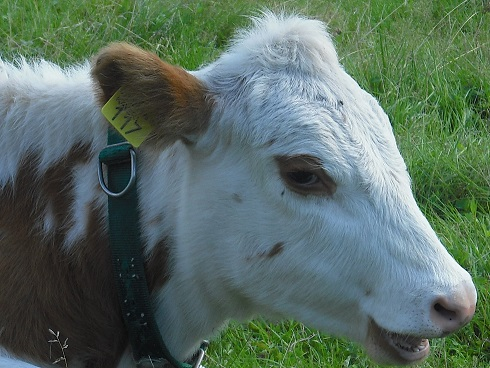
\includegraphics[width = 4cm,angle=90]{smile}
    \end{minipage}
    \begin{minipage}{5cm}
        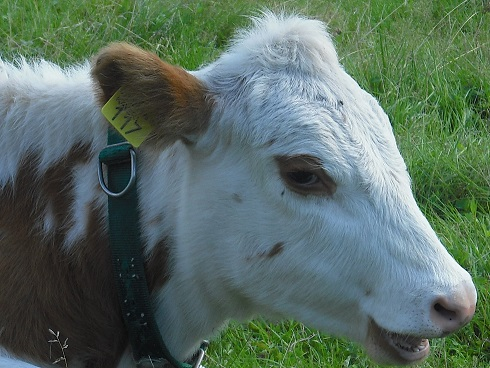
\includegraphics[height=4cm,angle=180]{smile}
    \end{minipage}

    Huomaa, että useammat määritteet erotetaan toisistaan pilkuilla!
\end{frame}
\begin{frame}[fragile]
    \begin{harj}
        Tallenna työkansioosi jokin kuva (tarkkana formaatin kanssa) ja tuo se työhösi sopivasti skaalattuna. Muista ottaa ensin käyttöön paketti \verb-graphicx-! 
    \end{harj}
\end{frame}
\subsubsection{Figure-ympäristö}
\begin{frame}[fragile]
    \frametitle{Kelluva figure-ympäristö}
    Käyttämällä pelkästään komentoa \verb-\includegraphics[]{}- kuva tuodaan komennon osoittamaan paikkaan, kuin osaksi tekstiä. Tämä näyttää käytännössä aina pahalta. 
    \vaihto
    On parempi antaa \LaTeX in päättää itse mihin kuva sijoitetaan eli tehdä kuvasta \emph{kelluva}. Tämä onnistuu käyttämällä \verb-figure--ympäristöä. 
\end{frame}
\begin{frame}[fragile]
    \frametitle{Kelluva kuva}
    \begin{scriptsize}
        \begin{Verbatim}[frame=single]
\begin{figure}[h!]
    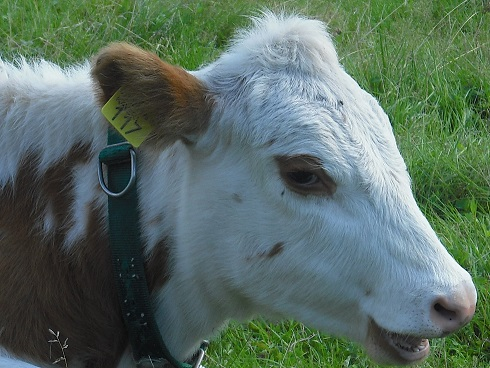
\includegraphics[height=4cm]{smile}
    \caption{Helppo hymyillä}
\end{figure}
        \end{Verbatim}
    \end{scriptsize}
    \begin{figure}[h!]
        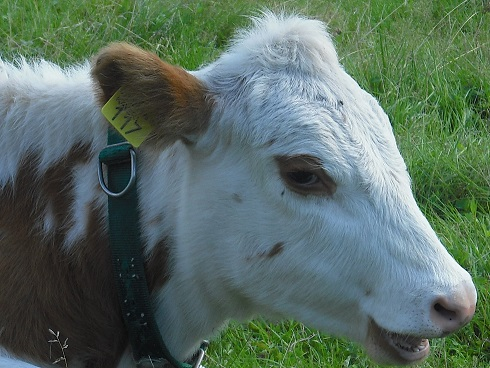
\includegraphics[height=4cm]{smile}
        \caption{Helppo hymyillä}
    \end{figure}
\end{frame}
\begin{frame}[fragile]
    \frametitle{Figure-ympäristön argumentit}
%    Kelluvalle ympäristölle (yllä \verb-figure-) voidaan antaa valinnaisena argumenttina toive kuvan sijoittamisesta. Toiveen voi esittää seuraavilla määritteillä:
    Oletuksena \LaTeX\ yrittää sijoittaa kelluvan ympäristön (yllä \verb-figure-) tekstisivun ylä- tai alareunaan tai sivulle, jolla on vain kelluvia olioita. Valinnaisella argumentilla voi kertoa tarkemmin, mihin kohtaan sijoittaminen sallitaan:
    \begin{table}
        \begin{tabular}{lcl}

            %h! && tähän\\
            %\hline
            h && salli sijoittaminen tähän (mahdollisesti keskelle sivua)\\
            \hline
            t && salli sijoittaminen sivun yläreunaan\\
            \hline
            b && salli sijoittaminen sivun alareunaan\\
            \hline
            p && salli sijoittaminen omalle sivulleen

        \end{tabular}
    \end{table}
    Oletuksena on siis \verb-[tbp]-. Argumenttina voi myös antaa huutomerkin, jolloin \LaTeX\ sallii rumempia lopputuloksia. Esimerkiksi \verb-[!hb]- sallii sijoittamisen tähän tai tekstisivun alareunaan ja tuloksen ei tarvitse näyttää yhtä hyvältä kuin jos argumenttina olisi vain \verb-[hb]-. Sijoittamista yritetään \emph{aina} järjestyksessä \verb-htbp-. Tarkempi kuvaus sijoittelualgoritmista: \url{http://tex.stackexchange.com/a/39020/23378}

\end{frame}
\begin{frame}[fragile]
    \frametitle{Figure-ympäristön argumentit}
    \begin{harj}
        Tuo työhösi jokin kuva käyttäen figure-ympäristöä ja anna valinnaisena argumenttina toiveesi kuvan sijoittamisesta. Lisää vielä kuvateksti.
    \end{harj}
\end{frame}
\subsubsection{Piirtäminen (TikZ)}
\begin{frame}[fragile]
    \frametitle{Kuvien piirtäminen}
    Kuvien liittämisen lisäksi niitä voi myös piirtää suoraan \LaTeX illa. Yksinkertaisimmissa tapauksissa tämä onnistuu helposti, monimutkaisempien kuvien tuottaminen vaatii harjaantumista.
    \vaihto
    Kuvien piirtäminen vie aikaa, mutta jälki on sen mukaista eikä erillisiä kuvatiedostoja tarvitse säilyttää.
    \vaihto Kuvien piirtämistä varten on tarjolla muutamia paketteja, joista erityisesti \verb-TikZ- on syytä mainita. 
    \verb-TikZ-illä kuvien piirtäminen tapahtuu ikään kuin pikseli kerrallaan, joten tarkkuus on verraton. 
    \vaihto Geogebra osaa kääntää sillä luodut kuvat \verb-tikz--koodiksi, mikä helpottaa työtä valtavasti.
    \vaihto Muita kuvien tuottamiseen tarkoitettuja paketteja ovat picture, xy-Pic ja Asymptote.
\end{frame}
\begin{frame}[fragile]
    \begin{harj}
    Piirrä Geogebralla jokin yksinkertainen kuva (vältä funktioita). Rajaa kuva sopivasti ja valitse File > Export > Graphics View as PGF/TikZ. Luo koodi ja kopioi siitä tarvittavat osat tiedostoosi. Tarvittavia osia ovat esittelyosan komennot \verb-\usepackage...-, \verb-\usetikzlibrary...-, mahdolliset värien määrittelyt \verb-\definecolor...- ja varsinainen kuva, eli \verb-\begin{tikzpicture}...\end{tikzpicture}-. 
    \end{harj}
    \begin{harj}\label{kelluvaTikz}
        Kopioi edellisessä harjoituksessa luomasi kuvan koodi ja tee kuvaan joitakin muutoksia pelkästään koodia muuttamalla. Voit esimerkiksi vaihtaa jonkin pisteen paikkaa tai piirtää kokonaan uutta. Tee uudesta kuvasta kelluva ja keksi jokin kuvateksi. 
    \end{harj}

\end{frame}
\subsection{Taulukot}
\begin{frame}[fragile]
    \frametitle{Taulukot}
    Taulukoiden rakentaminen \LaTeX issa on oma taiteenlajinsa. Mahdollisuudet ovat rajattomat, mutta perusteiden opettelu vaatii hieman energiaa. 
    \vaihto
Perinteisin tapa on käyttää \verb-tabular--ympäristöä. Tällöin taulukon sisältö kirjoitetaan komentojen \verb-\begin{tabular}[]{}- ja \verb-\end{tabular}- väliin.
    \vaihto
    Ympäristöllä on pakollinen argumentti, jolla määritellään taulukon asetukset, eli miten kunkin sarakkeen sisältö tasataan ja millaisia pystyviivoja käytetään.
\end{frame}
%\begin{frame}[fragile]

%\frametitle{Taulukot}
%Komento 
%\begin{Verbatim}[frame=single]
%\begin{tabular}{cc|c}
%-1 & 2 & 3,142\\
%4 & 5 & -6\\
%0 & 0 & 0
%\end{tabular}
%\end{Verbatim}
%luo taulukon, jossa on yksi pystyviiva ja jonka jokaisen sarakkeen sisältö on keskitetty:
%\begin{framed} 
%\begin{tabular}{cc|c}
%-1 & 2 & 3,142\\
%4 & 5 & -6\\
%0 & 0 & 0
%\end{tabular}
%\end{framed}
%Huomaa, ettei asetuksissa oteta kantaa rivien määrään.
%\end{frame}
\subsubsection{Tabular-ympäristö}
\begin{frame}[fragile]
    \frametitle{Tabular-ympäristö}
    Tabular-ympäristön pakollinen argumentti on jono seuraavia merkkejä:
    \begin{table}[h!]
        \begin{scriptsize}
            \begin{tabular}{ccp{5cm}}
                Merkki && Toiminto\\
                \hline
                \verb-r- && sarakkeen sisällön tasaus oikealle\\
                \hline
                \verb-l- && sarakkeen sisällön tasaus vasemmalle\\
                \hline
                \verb-c- && sarakkeen sisällön keskitys\\
                \hline
                \verb-|- && pystyviivan paikka\\
                \hline
                \verb-||- && kaksi pystyviivaa\\
                \hline
                \verb-p{'pituus'}- && pituus, jonka jälkeen rivi katkaistaan\\
                \hline
            \end{tabular}
        \end{scriptsize}
    \end{table}
    Esimerkiksi komento \verb-\begin{tabular}{r|cc}- aloittaisi 3-sarakkeisen taulukon, jolla olisi pystyviiva 1. ja 2. sarakkeen välillä. Sarakkeen 1 sisältö tasattaisiin oikealle, kahden muun sisältö keskitettäisiin.
    %\vaihto
    %Lisätietoja ympäristön käytöstä saa kirjasta  \begin{scriptsize}\url{http://en.wikibooks.org/wiki/LaTeX/Tables#The_tabular.2A_environment}\end{scriptsize}
\end{frame}

\begin{frame}[fragile]
    \frametitle{Tabular-ympäristö}
    Taulukon sisältö kirjoitetaan rivi kerrallaan. Jokaisella rivillä merkki \verb-&- erottaa sarakkeet toisistaan, komennolla \verb-\\- siirrytään seuraavalle riville.  Nämä ja muut taulukon sisäiset komennot ovat seuraavassa:
    \vaihto
    \begin{table}[h!]
        \begin{scriptsize}
            \begin{tabular}{cp{4cm}}
                Komento & Toiminto\\
                \hline
                \verb-&- & sarakkeenvaihto\\
                \hline
                \verb-\\- & rivinvaihto\\
                \hline
                \verb-\hline- & vaakaviiva \\
                \hline
                \verb-\newline- & rivinvaihto sarakkeen sisällä\\
                \hline
                \verb+\cline{i-j}+ & vaakaviiva sarakkeiden i ja j välillä\\
                \hline
            \end{tabular}
        \end{scriptsize}
    \end{table}

\end{frame}

\begin{frame}[fragile]
    \frametitle{Tabular-ympäristö}
    Esimerkiksi rivi
    \begin{scriptsize}
        \begin{Verbatim}[frame=single]
\begin{tabular}{r|cc}
    & Tytöt & Pojat\\
    \hline
    Sinisilmäiset & 4 & 2 \\
    Ruskeasilmäiset & 3 & 5 \\
    Vihreäsilmäiset & 8 & 8\\
\end{tabular}
        \end{Verbatim}
    \end{scriptsize}
    luo seuraavan taulukon:
    \begin{framed} 
        \begin{tabular}{r|cc}
            & Tytöt & Pojat\\
            \hline
            Sinisilmäiset & 4 & 2 \\
            Ruskeasilmäiset & 3 & 5 \\
            Vihreäsilmäiset & 8 & 8\\
            %\hline
            %Yhteensä: & 15 & 15\\
        \end{tabular}
    \end{framed}
    Huomaa, ettei rivien lukumäärää tarvitse erikseen kertoa \LaTeX ille.

\end{frame}



\begin{frame}[fragile]
    \frametitle{Tabular-ympäristö}
    \begin{harj}
        Laadi jokin 3-sarakkeinen taulukko, jossa on ainakin kaksi riviä.  
        %ja joka sisältää
        %\begin{itemize}
        %\item pystyviivan
        %\item kaksinkertaisen pystyviivan
        %\item vaakaviivan
        %\item osittaisen vaakaviivan sarakkeiden 1 ja 2 välillä
        %\end{itemize}
    \end{harj}
    \begin{harj}
        Luo toinen 3-sarakkeinen taulukko (esim. kopio edellisestä), joka sisältää 
        \begin{itemize}
            \item pystyviivan
            \item kaksinkertaisen pystyviivan
            \item vaakaviivan
            \item osittaisen vaakaviivan kahden sarakkeen välillä
        \end{itemize}
    \end{harj}
\end{frame}
\subsubsection{Sarakkeiden yhdistäminen}
\begin{frame}[fragile]
    \frametitle{Sarakkeiden yhdistäminen}
    Sarakkeiden yhdistäminen onnistuu komennolla \verb-\multicolumn{}{}{}-. Pakollisista argumenteista
    \begin{itemize}
        \item ensimmäinen on yhdistettävien solujen lukumäärä
        \item toinen on yhdistämällä saadun sarakkeen tasaus
        \item kolmas on yhdistämällä saadun sarakkeen sisältö
    \end{itemize}
    Komento \verb-\multicolumn- toimii sellaisenaan eikä tarvitse lisäpaketteja.
\end{frame}
\begin{frame}[fragile]
    \frametitle{Sarakkeiden yhdistäminen}
    %\begin{minipage}{5cm}
    \begin{scriptsize}
        \begin{Verbatim}[frame=single]
\begin{tabular}{|c|c|c|}
    \hline
    \multicolumn{3}{|c|}{3 yhdistettyä saraketta}\\
    \hline
    Sarake & \multicolumn{2}{c|}{2 yhdistettyä saraketta}\\
    \hline
    Sarake1 & Sarake2 & Sarake3\\
    \hline
\end{tabular}
        \end{Verbatim}
    \end{scriptsize}
    %\end{minipage}
    \begin{minipage}{5cm}
        \begin{scriptsize}
            \begin{tabular}{|c|c|c|}
                \hline
                \multicolumn{3}{|c|}{3 yhdistettyä saraketta}\\
                \hline
                Sarake & \multicolumn{2}{c|}{2 yhdistettyä saraketta}\\
                \hline
                Sarake1 & Sarake2 & Sarake3\\
                \hline
            \end{tabular}
        \end{scriptsize}
    \end{minipage}
\end{frame}

\begin{frame}[fragile]
    \frametitle{Sarakkeiden yhdistäminen}

    \begin{harj}
        Luo seuraava taulukko:
        \begin{table}
            \begin{tabular}{|l|l|l|}
                \hline
                \multicolumn{3}{|c|}{\Large Päiväpetolintuja}\\
                \hline
                \textit{Nimitys} & \textit{Suku} & \textit{Laji}\\ \hline
                Kanahaukka & Accipiter &  gentilis\\ \hline
                Hiirihaukka & Buteo & buteo\\ \hline
                %\multicolumn{3}{|c|}{Jalohaukkoja}\\ \hline
                Tuulihaukka & Falco & columbarius\\\hline
                Nuolihaukka & Falco & subbuteo\\ \hline
            \end{tabular}
        \end{table}
    \end{harj}

\end{frame}
\subsubsection{Rivien yhdistäminen}
\begin{frame}[fragile]
    \frametitle{Rivien yhdistäminen}
    Rivien yhdistämistä varten tarvitaan paketti \verb-multirow-. Tämän käyttöönottamisen jälkeen rivien yhdistäminen (sarakkeen sisällä) onnistuu komennolla \verb-\multirow{}{}{}-. Pakollisista argumenteista
    \begin{itemize}
        \item ensimmäinen on yhdistettävien solujen lukumäärä
        \item toinen on yhdistämällä saadun rivin leveys (\verb-*- jättää asian \LaTeX in huoleksi)
        \item kolmas on yhdistämällä saadun rivin sisältö
    \end{itemize}
    Rivin leveyttä ei useinkaan kannata itse valita, ellei ole varma siitä mitä haluaa tehdä. 
    \vaihto
    Huomaa, että \verb-\multirow- toimii kuten \verb-\multicolumn-, mutta keskimmäinen argumentti on eri tarkoitusta varten.
\end{frame}
\begin{frame}[fragile]
    \frametitle{Rivien yhdistäminen} 
    \begin{scriptsize}
        \begin{Verbatim}[frame=single]
\begin{tabular}{|c|c|c|}
    \hline
    \multirow{3}{*}{Kolme riviä} & Solu1 & Solu 2\\
    \cline{2-3}
    & \multirow{2}{*}{Kaksi riviä} & Solu 3\\
    \cline{3-3}
    & & Solu 4\\
    \hline
\end{tabular}
        \end{Verbatim}
    \end{scriptsize}
    \begin{tabular}{|c|c|c|}
        \hline
        \multirow{3}{*}{Kolme riviä} & Solu1	& Solu 2\\\cline{2-3}
                                      & \multirow{2}{*}{Kaksi riviä}	& Solu 3\\\cline{3-3}
                                      & & Solu 4\\
        \hline
    \end{tabular}
\end{frame}
\begin{frame}[fragile]
    \frametitle{Rivien yhdistäminen} 
    \begin{harj}
        Luo seuraava taulukko: 
        \begin{table}\label{taulukko}
            \begin{tabular}{|c|c|c|c|}
                \hline
                \textit{Heimo} & \textit{Nimitys} & \textit{Suku} & \textit{Laji}\\ \hline
                \multirow{2}{*}{Haukat} & Kanahaukka & Accipiter &  gentilis\\ \cline{2-4}
                                        & Hiirihaukka & Buteo & buteo\\ \hline
                %\hline
                %Analyysi I \& II & \multirow{3}{*}{Matikan perusopinnot}\\
                %\cline{1-1}
                %Linis I & \\
                %\cline{1-1}
                %JYM & \\
                %\hline
            \end{tabular}
        \end{table}
    \end{harj}
\end{frame}
\begin{frame}[fragile]
    \frametitle{Sarakkeiden ja rivien yhdistäminen} 
    Sarakkeita ja rivejä voi yhdistää samassa taulukossa:\vaihto
    \begin{minipage}{8cm}
        \begin{scriptsize}
            \begin{verbatim}
\begin{tabular}{|l|l|l|l|}
    \hline
    \multicolumn{4}{|c|}{\Large Päiväpetolintuja}\\
    \hline
    \textit{Heimo} & \textit{Nimitys} & \textit{Suku} & \textit{Laji}\\
    \hline
    \multirow{2}{*}{Haukat} & Kanahaukka & Accipiter &  gentilis\\
                              \cline{2-4}
                            & Hiirihaukka & Buteo & buteo\\
    \hline
    \multirow{2}{*}{Jalohaukat} & Tuulihaukka & Falco & columbarius\\
                                  \cline{2-4}
                                & Nuolihaukka & Falco & subbuteo\\
    \hline
\end{tabular}
            \end{verbatim}
        \end{scriptsize}
    \end{minipage}
    \begin{table}[h!]
        \begin{scriptsize}
            \begin{tabular}{|l|l|l|l|}
                \hline
                \multicolumn{4}{|c|}{\Large Päiväpetolintuja}\\
                \hline
                \textit{Heimo} & \textit{Nimitys} & \textit{Suku} & \textit{Laji}\\\hline
                \multirow{2}{*}{Haukat} & Kanahaukka & Accipiter &  gentilis\\ \cline{2-4}
                                        & Hiirihaukka & Buteo & buteo\\ \hline
                \multirow{2}{*}{Jalohaukat} & Tuulihaukka & Falco & columbarius\\ \cline{2-4}
                                            &Nuolihaukka & Falco & subbuteo\\ \hline
            \end{tabular}
        \end{scriptsize}
    \end{table}

\end{frame}
\begin{frame}
    Taulukoiden rakentamisessa lähes mikä tahansa on mahdollista. Kirjasta \url{http://en.wikibooks.org/wiki/LaTeX/Tables} voi etsiä apua monimutkaisempia toteutuksia varten.
\end{frame}
%\begin{frame}[fragile]
%\frametitle{Kelluvat taulukot}
%Yleensä taulukot kannattaa esittää kelluvina ympäristöinä. Tämä tarkoittaa sitä, että \LaTeX\ päättää itse, mihin taulukko kannattaa ulkonäöllisesti sijoittaa. Tällöin \verb-tabular--ympäristö sijoitetaan \verb-table--ympäristöön:
%
%\end{frame}
%\begin{frame}[fragile]
%\frametitle{Kelluvat taulukot}
%\verb-table--ympäristölle voidaan antaa valinnaisena argumenttina toive taulukon sijoittumisesta seuraavilla määritteillä:
%\begin{tabular}{cc}
%h! & tähän\\
%h & suunnilleen tähän\\
%b & sivun alareunaan\\
%p & sivun yläreunaan
%\end{tabular}
%\end{frame}
\subsubsection{Kelluva table-ympäristö}
\begin{frame}[fragile]
    \frametitle{Kelluva table-ympäristö}
Komento \verb-\begin{tabular}{...}...\end{tabular}- luo taulukon komennon osoittamaan paikkaan, kuin osaksi tekstiä. Tämä näyttää käytännössä aina pahalta. 
    \vaihto
    On parempi antaa \LaTeX in päättää itse mihin taulukko sijoitetaan eli tehdä siitä \emph{kelluva}. Tämä onnistuu sijoittamalla taulukko \verb-table--ympäristöön.
    \begin{Verbatim}[frame=single]
\begin{table}
    \begin{tabular}{...}
        ...
    \end{tabular}
\end{table}
    \end{Verbatim}
    Kuten \verb-figure--ympäristöllä, \verb-table- yritetään oletuksena sijoittaa tekstisivun ylä- ja alareunaan tai kelluvien olioiden sivulle. Sijoitteluun voi vaikuttaa antamalla \verb-table--ympäristölle valinnaisena argumenttina osan tai kaikki merkeistä \verb-!htbp-.
\end{frame}
%\begin{frame}[fragile]
%    \frametitle{Table-ympäristön argumentit}
%    Kelluvalle ympäristölle (yllä \verb-table-) annetaan valinnaisena argumenttina toive taulukon sijoittamisesta. Toiveen voi esittää seuraavilla määritteillä:
%    \begin{table}
%        \begin{tabular}{lcl}
%
%            h! && tähän\\
%            \hline
%            h && suunnilleen tähän\\
%            \hline
%            b && sivun alareunaan\\
%            \hline
%            t && sivun yläreunaan\\
%            \hline
%            p && omalle sivulleen\\
%
%        \end{tabular}
%    \end{table}
%    Toive ei ole \LaTeX in tärkeysjärjestyksessä korkeimmalla, joten se ei aina toteudu.
%\end{frame}
\begin{frame}[fragile]
    \begin{harj}\label{kelluvaTaulukko}
        Tee tehtävässä \ref{taulukko} luomastasi taulukosta kelluva ja anna sille jokin nimi. Kokeile erilaisia sijoitteluvaihtoehtoja. Lisää koodiisi kommenttirivi, jossa kerrot valintasi. 
    \end{harj}

\end{frame}
\subsection{Matriisit}
\begin{frame}[fragile]
    \frametitle{Matematiikkatilan taulukot}
    \LaTeX\ olettaa \verb-tabular--ympäristön sisältävän tavallista tekstiä. Taulukoituja matemaattisia ilmaisuja varten on oma ympäristönsä \verb-array-. Sitä käytetään kuten \verb-tabular--ympäristöä, mutta se täytyy sijoittaa matematiikkatilaan.\vaihto

    \begin{minipage}{5cm}
        \begin{scriptsize}
            \begin{Verbatim}[frame=single]
\[
    \begin{array}{r|c}
        x & x^2+1\\
        \hline
        -1 & 2\\
        0 & 1\\
        1 & 2\\
    \end{array}
\]
            \end{Verbatim}
        \end{scriptsize}
    \end{minipage}
    \begin{minipage}{3cm}
        \[
        \begin{array}{r|c}
            x & x^2+1\\
            \hline
            -1 & 2\\
            0 & 1\\
            1 & 2\\
        \end{array}
        \]
    \end{minipage}
\end{frame}
\begin{frame}[fragile]
    \frametitle{Array-ympäristö}
    Array-ympäristöllä voi kirjoittaa esimerkiksi paloittain määritellyn funktion lausekkeen. Tämän voi toteuttaa lyhyemminkin käyttäen ympäristöä \verb-cases-. 
    \begin{Verbatim}[frame=single]
\[
    f(x) =
    \begin{cases}
        x,  & \text{kun } x>0,\\
        -x, & \text{kun } x\leq0.
    \end{cases}
\]
    \end{Verbatim}
    \begin{framed}
        \[
            f(x) =
            \begin{cases}
                x,  & \text{kun } x>0,\\
                -x, & \text{kun } x\leq0.
            \end{cases}
        \]
    \end{framed}
\end{frame}
\subsubsection{Matriisiympäristöt}
\begin{frame}[fragile]
    \frametitle{Matriisit}
    Matriisit voitaisiin luoda käsin käyttäen \verb-array--ympäristöä, mutta hieman helpompiakin tapoja on. Esimerkiksi ympäristöllä \verb-pmatrix- matriiseja luotaisiin seuraavasti:

    \begin{minipage}{4cm}
        \begin{scriptsize}
            \begin{Verbatim}[frame=single]
\[
    \begin{pmatrix}
        a & b & c\\
        1 & 2 & 3\\
    \end{pmatrix}
\]
            \end{Verbatim}
        \end{scriptsize}
    \end{minipage}
    \begin{minipage}{4cm}
        \[
            \begin{pmatrix}
                a & b & c\\
                1 & 2 & 3\\
            \end{pmatrix}
        \]
    \end{minipage}

Syntaksi on siis samanhenkinen kuin ympäristöllä \verb-array-, mutta sarakkeiden määrää ei tarvitse kertoa erikseen. Virheiden varalta muista, että
    \begin{itemize}
        \item sarakkeet erotetaan toisistaan komennolla \verb-&-
        \item rivi vaihdetaan komennolla \verb-\\-
    \end{itemize}

    %\end{frame}
    %\begin{frame}[fragile]
    %
    %\end{frame}
    %loisi matriisin
%Saman voi kuitenkin tehdä helpommin käyttämällä matriiseja varten luotuja ympäristöjä, kuten \verb-bmatrix*- tai \verb-pmatrix*-. Näitä varten tarvitset paketin \verb-mathtools-.
\end{frame}
\begin{frame}[fragile]
    \begin{harj}
        Luo jokin vähintään \(2\times 3\)-matriisi käyttäen ympäristöä \verb-pmatrix-, kuten yllä. Tee sitten matriisistasi muutama kopio ja kokeile ympäristöjä \verb-matrix-, \verb-bmatrix- ja \verb-vmatrix-. (Kunkin kohdalle kannattaa kirjoittaa kommentti tulostuvan matriisin tyylistä.)
    \end{harj}
\end{frame}
\begin{frame}[fragile]
    \frametitle{Matriisit}
    Vaikka ympäristöt \verb-pmatrix- (\verb-matrix-, \verb-bmatrix-, \verb-vmatrix-) pohjautuvat \verb-array--ympäristöön, ei sarakkeiden tasaukseen voi lähtökohtaisesti vaikuttaa. \vaihto Paketti \verb-mathtools- tarjoaa vastaavat ympäristöt \verb-pmatrix*-, \verb-bmatrix*- jne., joilla on valinnaisena argumenttina sarakkeissa käytetty tasaus:\vaihto

    \begin{minipage}{4cm}
        \begin{scriptsize}
            \begin{Verbatim}[frame=single]
\[
    \begin{pmatrix*}[r]
        a & b & c\\
        -1 & -2 & -3\\
    \end{pmatrix*}
\]
            \end{Verbatim}
        \end{scriptsize}
    \end{minipage}
    \begin{minipage}{4cm}
        \[
            \begin{pmatrix*}[r]
                a & b & c\\
                -1 & -2 & -3\\
            \end{pmatrix*}
        \]
    \end{minipage}
    %Seuraavaan taulukkoon on koottu yleisimmin tarvittavat matriisiympäristöt:
    %\vaihto
    %\begin{tabular}{|c|c|}
    %\hline
    %Ympäristön nimi & Matriisin tyyli\\[0.3em]
    %\hline
    %\verb-matrix*- & $\begin{smallmatrix}a&b\\ c&d\end{smallmatrix}$\\[0.3em]
    %\verb-pmatrix*- & $\bigl(\begin{smallmatrix}a&b\\ c&d\end{smallmatrix} \bigr)$\\[0.3em]
    %\verb-bmatrix*- & $\bigl[\begin{smallmatrix}a&b\\ c&d\end{smallmatrix} \bigr]$\\[0.3em]
    %\verb-vmatrix*- & $\left|\begin{smallmatrix}a&b\\ c&d\end{smallmatrix} \right|$\\[0.3em]
    %\hline
    %\end{tabular}
    %\vaihto
    %Ympäristöllä on valinnainen argumentti, jolla valitaan tekstin tasaus (r, l tai c). Jos ympäristön nimestä jätetään * pois, sarakkeiden sisältö keskitetään (tällöin pakettia \verb-mathtools- ei tarvita). 
\end{frame}
\begin{frame}[fragile]
    \frametitle{Matriisit}

    Esimerkki:\vaihto
    \begin{minipage}{5cm}
        \begin{scriptsize}
            \begin{Verbatim}[frame=single]
\[
    \begin{bmatrix*}[r]
        -1 & 2\\
        0 & 1\\
        1 & -2\\
    \end{bmatrix*}^T = 
    \begin{bmatrix*}[r]
        -1 & 0 & 1\\
        2 & 1 & -2
    \end{bmatrix*}
\]
            \end{Verbatim}
        \end{scriptsize}
    \end{minipage}
    \begin{minipage}{5cm}
        \[
        \begin{bmatrix*}[r]
            -1 & 2\\
            0 & 1\\
            1 & -2\\
        \end{bmatrix*}^T = 
        \begin{bmatrix*}[r]
            -1 & 0 & 1\\
            2 & 1 & -2
        \end{bmatrix*}
        \]
    \end{minipage}
\end{frame}
\begin{frame}[fragile]
    \frametitle{Matriisit}
    \begin{harj}
        Kirjoita seuraavanlainen matriisitoimitus: 
        \begin{align*}
            &
            \begin{bmatrix*}[r]
                0 & 0 & 1 & a_1\\
                0 & 1 & 1 & a_2\\
                1 & 1 & 1 & a_3
            \end{bmatrix*}
%        \stackrel{\begin{scriptsize} R_1\leftrightarrow R_3 \end{scriptsize} }{\longrightarrow}
        \xrightarrow{R_1\leftrightarrow R_3}
            \begin{bmatrix*}[r]
                1 & 1 & 1 & a_3\\
                0 & 1 & 1 & a_2\\
                0 & 0 & 1 & a_1
            \end{bmatrix*}
            %\\
            %\stackrel{\begin{scriptsize} R_1-R_2 \end{scriptsize} }{\longrightarrow}
            %&\begin{bmatrix*}[r]
            %1 & 0 & 0 & a_3-a_2\\
            %0 & 1 & 1 & a_2\\
            %0 & 0 & 1 & a_1
            %\end{bmatrix*}
            %\stackrel{\begin{scriptsize} R_2-R_3 \end{scriptsize} }{\longrightarrow}
            %\begin{bmatrix*}[r]
            %1 & 0 & 0 & a_3-a_2\\
            %0 & 1 & 0 & a_2-a_1\\
            %0 & 0 & 1 & a_1
            %\end{bmatrix*}
        \end{align*}
        Matriisien sisällön saat päättää vapaasti eikä rivitoimituksen tarvitse mennä oikein. % Matriisien välisen merkinnän saat rakennettua komennon \verb-\stackrel{}{}- avulla. Yllä on käytetty komentoa
        Kaavan mukana automaattisesti venyvän nuolen saa komennolla \verb-\xrightarrow{kaava}-.
%        \begin{verbatim}
%        \stackrel{
%            \begin{scriptsize} 
%                R_1\leftrightarrow R_3 
%            \end{scriptsize}
%        }{\longrightarrow} 
%        \end{verbatim}

        % Kannattaa kopioida alkuperäisen matriisin koodi ja muokata sitä kunkin uuden matriisin kohdalla. Matriisit vievät paljon tilaa, joten ympäristö \verb-align*- on hyödyksi!
    \end{harj}
\end{frame}
\subsubsection{Lisätietoa}
\begin{frame}[fragile]
    \frametitle{Lisätietoa matriiseista}
    Tavalliset matriisiympäristöt \verb-pmatrix- jne. voidaan säätää noudattamaan paremmin \verb-array--ympäristön syntaksia.
    \vaihto
    Tämä on tarpeen, jos halutaan valita eri sarakkeisiin erilainen tasaus tai luoda pystyviiva matriisin sisälle. 
    \vaihto
    Syntaksin muuttaminen onnistuu kopioimalla esittelyosaan komennot\vaihto
    \begin{Verbatim}[frame=single]
\makeatletter
\renewcommand*\env@matrix[1][*\c@MaxMatrixCols c]{%
    \hskip -\arraycolsep
    \let\@ifnextchar\new@ifnextchar
\array{#1}}
\makeatother
    \end{Verbatim}
\end{frame}
\begin{frame}[fragile]
    \frametitle{Lisätietoa matriiseista}
    Edellä tehtyjen muutosten jälkeen matriisiympäristöt toimivat kuten ennenkin, mutta lisäksi valinnainen argumentti on käytössä kuten \verb-array--ympäristöllä:
    \vaihto
    \begin{minipage}{4.2cm}
        \begin{scriptsize}
            \begin{Verbatim}[frame=single]
\[
    \begin{bmatrix}[rrr|r]
        0 & 0 & 1 & -a_1\\
        0 & 1 & -1 & a_2\\
        1 & 1 & 1 & a_3
    \end{bmatrix}
\]
            \end{Verbatim}
        \end{scriptsize}
    \end{minipage}
    \begin{minipage}{4cm}
        \[
            \begin{bmatrix}[rrr|r]
                0 & 0 & 1 & -a_1\\
                0 & 1 & -1 & a_2\\
                1 & 1 & 1 & a_3
            \end{bmatrix}
        \]
    \end{minipage}
\end{frame}


\section{4.kerta}
\subsection{Viittaaminen kuviin ja taulukoihin}
\begin{frame}[fragile]
    \frametitle{Viittaaminen kuviin ja taulukoihin}
    Kelluviksi kirjoitetut kuvat ja taulukot tulevat numeroiduiksi, jolloin niihin viittaaminen onnistuu helposti komennoilla \verb-\label{}- ja \verb-\ref{}-. 
    %\begin{itemize}
    %\item \verb-\ref{nimi}- (tulostaa viitattavan kohteen numeron)
    %\item \verb-\eqref{nimi}- (tulostaa kohteen numeron sulkujen sisällä)
    %\item \verb-\pageref{nimi}- (tulostaa sen sivun numeron, jolla kohde on)  
    %\end{itemize}
    %Sisäisten viittausten kanssa tulee aina käyttää komentoja. Tällöin viittaukset pysyvät kohdallaan vaikka numeroinnit muuttuisivat työn edetessä.
    %\end{frame}
    %\begin{frame}[fragile]
    %Huom! Uuden viittauksen jälkeen työn joutuu ajamaan kahdesti, jotta numeroinnit tulevat näkyviin (kahden kysymysmerkin sijaan).
    \begin{harj}
        Viittaa harjoituksessa \ref{kelluvaTaulukko} luomaasi kelluvaan taulukkoon. Käytä komentoja \verb-\ref{}- ja \verb-\pageref{}-. Komento \verb-\label- tulee taulukkoon liittyvän \verb-\caption{..}--komennon jälkeen.
        \vaihto
        %Muista, että viitattavalle kohteelle on ensin annettava tunnus komennolla \verb-\label{valitsemasi tunnus}-. Komento sijoitetaan ympäristön aloittavan komennon \verb-\begin{}- perään.
    \end{harj}
    \begin{harj}
        Sama kuin edellinen harjoitus, mutta viittaa harjoituksessa \ref{kelluvaTikz} luomaasi kelluvaan kuvaan.
    \end{harj}
\end{frame}
\subsection{Kirjallisuusviitteet}
\subsubsection{Lainaukset ja alaviitteet}
\begin{frame}[fragile]
    \frametitle{Lainaukset ja alaviitteet}
    Suomalaisittain käytettävät lainausmerkit saa kahdella peräkkäisellä \verb-'- merkillä:
    \begin{Verbatim}[frame=single]
Matti sanoi: ''Onpa outoa!''
    \end{Verbatim}
    tulostaa
    \begin{framed}
        Matti sanoi: ''Onpa outoa!''
    \end{framed}
    Lainauksia varten on olemassa myös omia ympäristöjään, kuten \verb-verse-, \verb-quote- ja \verb-quotation-.
    \vaihto
    Alaviitteen voi luoda komennolla \verb-\footnote{teksti}-. Komento kirjoitetaan siihen kohtaan, johon alaviitteen merkki halutaan. 
\end{frame}
\begin{frame}[fragile]
    \begin{harj}
        Lisää dokumenttiisi jokin lainaus käyttäen \verb-quote--, \verb-\quotation-- tai \verb-verse--ympäristöä. 
    \end{harj}
    \begin{harj}
        Lisää työhösi alaviite komennolla \verb-\footnote{}-. 
    \end{harj}
\end{frame}
\subsubsection{BibTeX-järjestelmä}
\begin{frame}[fragile]
    \frametitle{Kirjallisuusviitteet}
    \LaTeX issa kirjallisuusviittaukset kannattaa hoitaa \(\BibTeX\)-järjestelmän avulla. 
    \vaihto
%    Tällöin jokaista lähdeteosta kohden luodaan erillinen \verb-.bib--tiedosto, joka sisältää teoksen tiedot. 
    Tällöin lähdeteokset kirjataan erilliseen \verb-.bib--tiedostoon (tai -tiedostoihin).
    \vaihto
    Tiedostot on yksinkertaisinta tallentaa samaan kansioon \verb-.tex--tiedoston kanssa.
    \vaihto
    Viittaaminen tapahtuu komennolla \verb-\cite{tunnus}-, jossa \verb-tunnus- on eräs \verb-.bib--tiedostosta löytyvä merkkijono.
    %\vaihto
    %Aivan työn loppuun luodaan kirjallisuusluettelo komennoilla
    %\begin{Verbatim}[frame=single]
    %\bibliographystyle{luettelon tyyli}
    %\bibliography{teos1.bib, teos2.bib, teos3.bib,...}
    %\end{Verbatim}
    %Edellytyksenä on, että tiedostot teos1.bib jne. ovat samassa kansiossa \verb-.tex--tiedoston kanssa.
\end{frame}
\begin{frame}[fragile]
    \frametitle{.bib-tiedostot}
    \verb-.bib--tiedoston voi luoda millä tahansa tekstieditorilla, erityisen hyvin Texmakerilla. 
    \vaihto
    Tiedoston sisältö voisi olla esimerkiksi seuraava:\vaihto
    \begin{scriptsize}
        \begin{Verbatim}[frame=single]
@book{kemper,
    title={A Course in Commutative Algebra},
    author={Kemper, G.},
    isbn={9783642035456},
    series={Graduate Texts in Mathematics},
    url={http://books.google.fi/books?id=8kxlj48DWM4C},
    year={2010},
    publisher={Springer Berlin Heidelberg}
}
        \end{Verbatim}
    \end{scriptsize}
    %Tiedosto tallennetaan muodossa \verb-jokinNimi.bib- samaan kansioon \verb-.tex--tiedoston kanssa (ei pakollista, mutta yksinkertaisinta).
\end{frame}
\begin{frame}[fragile]
    \frametitle{.bib-tiedostot}
    \begin{harj}
        Kopioi edellisen esimerkin sisältö uuteen tiedostoon ja tallenna se nimellä \verb-lahteet.bib- työkansioosi. 
    \end{harj}
\end{frame}
\begin{frame}[fragile]
    \frametitle{.bib-tiedoston sisältö}
    \begin{itemize}
        \item Ensimmäisellä komennolla (\verb-@book-, \verb-@article-, \verb-@unpublished- jne) kerrotaan, minkä tyyppisestä teoksesta on kyse. 
        \item Aaltosulkeisiin ennen ensimmäistä pilkkua tuleva merkkijono on se tunnus, jolla teokseen viitataan komennolla \verb-\cite{tunnus}-. 
        \item Tunnuksen voi valita vapaasti (ilman ääkkösiä ja erikoismerkkejä) eikä se tule näkyviin mihinkään.  Esimerkiksi yllä tunnus on \verb-kemper-, joten teokseen viitattaisiin komennolla \verb-\cite{kemper}-.
        \item Muut kentät (ja niiden pakollisuus/valinnaisuus) määräytyvät teoksen tyypin mukaan.
    \end{itemize}
\end{frame}
\begin{frame}[fragile]
    \frametitle{Luokat ja .bib-tiedoston sisältö}
    Kun tiedostoja luodaan käsin, täytyy selvittää mitkä kentät ovat pakollisia ja mitkä valinnaisia. 
    \vaihto
    Esimerkiksi taulukosta 
    \begin{scriptsize}
        \url{http://en.wikibooks.org/wiki/LaTeX/Bibliography_Management#Entry_and_field_types_in_.bib_files}
    \end{scriptsize}
    selviää, että kirjalle (\verb-@book-) pakollisia kenttiä ovat \verb-title- ja \verb-author-, muut valinnaisia.
    \vaihto
    Lisätietoa käytettävistä teosluokista löytyy esimerkiksi sivulta
    \begin{scriptsize}
        \url{http://en.wikibooks.org/wiki/LaTeX/Bibliography_Management#Standard_templates}.
    \end{scriptsize}
    \vaihto
    Käytännössä jokaista kuviteltavissa olevaa lähdeteosta varten löytyy jokin sopiva luokka (ja tarpeen tullen sellaisen voi luoda itsekin).
\end{frame}
\begin{frame}[fragile]
    \begin{harj}
        Lisää tiedostoon \verb-lahteet.bib- kirja, jonka nimi on Topologia I, kirjoittaja Jussi Väisälä, julkaisija Limes ry ja painovuosi 2000. Valitse viittaustunnukseksi \verb-topo1-.
    \end{harj}
\end{frame}
\begin{frame}[fragile]
    \frametitle{.bib-tiedostot Internetistä}
    Kirjojen teostietoja löytää \BibTeX -muodossa varsin suurella todennäköisyydellä Google Books-palvelusta. 
    \vaihto
    Kuhunkin teokseen liittyvän Tietoja teoksesta-sivun alalaidassa on kohta Vie sitaatti ja sen vieressä painike \BibTeX, josta tiedoston voi ladata.
    \vaihto
    Tiedosto kannattaa avata Texmakerillä, tehdä mahdolliset muutokset ja tallentaa haluttuun kansioon. 
    \vaihto
    Käytännössä ainakin viittaustunnus on syytä vaihtaa helpommaksi.
\end{frame}
\begin{frame}[fragile]
    \frametitle{.bib-tiedostot Internetistä}
    \begin{harj}
        Etsi Google Books-palvelusta Walter Rudinin kirjan Complex Analysis (kirjan versiolla ei väliä) tiedot \BibTeX -muodossa. Avaa tiedosto Texmakerilla ja valitse viittaustunnus haluamaksesi. Tallenna tiedosto nimellä \verb-Rudin.bib- työkansioosi. (Huomaa, että palvelu tarjoaa tiedostot muodossa .bibtex.)
    \end{harj}

\end{frame}
\begin{frame}[fragile]
    \frametitle{Kirjallisuusluettelon luominen}
    Kun tarvittavat \verb-.bib--tiedostot on tallennettu koneelle, on syytä luoda kirjallisuusluettelo. Kirjallisuusluetteloon tulee näkyviin ne teokset, joiden tiedot ovat olemassa ja joihin on viitattu ainakin kerran. Ei-viitatun teoksen saa lisättyä lähdeluetteloon \verb-\nocite{tunnus}--komennolla.
    \vaihto
    Luettelo luodaan työn loppuosaan komennolla
    \begin{Verbatim}[frame=single]
\bibliographystyle{luettelon tyyli}
\bibliography{lista1,lista2,lista3,...}
    \end{Verbatim}
    Koodissa \verb-listax- ovat \verb-.bib--tiedostojen nimet ilman \verb-bib--päätettä. Huomaa myös, ettei pilkun jälkeen sallita välilyöntiä.
    \vaihto
    Edellisen koodin toimimisen edellytyksenä on, että tiedostot \verb-lista1.bib- jne. ovat samassa kansiossa \verb-.tex--tiedoston kanssa. 
\end{frame}
\begin{frame}[fragile]
    \frametitle{Kirjallisuusluettelon luominen}
    \begin{harj}
        Edellä loit BibTeX-tiedostot \verb-lahteet.bib- ja \verb-Rudin.bib-. Tuo teokset kirjallisuusluetteloon koodilla 
        \begin{Verbatim}[frame=single]
\bibliographystyle{plain}
\bibliography{lahteet,Rudin}
        \end{Verbatim}
        Sijoita koodi työsi loppuosaan, esimerkiksi juuri ennen komentoa \verb-\end{document}-.
    \end{harj}
    \begin{harj}
        Viittaa kuhunkin teokseen työssäsi komennolla \verb-\cite{viittaustunnus}-.
    \end{harj}
\end{frame}
\begin{frame}[fragile]
    \frametitle{Käytäntö}
    %Kun tiedostot on luotu ja tallennettu, niihin voidaan viitata tuloksellisesti jo mainitulla komennolla \verb-\cite{tunnus}-. 
    Jotta viitteet tulisivat näkyviin, toimi seuraavasti:
    \begin{itemize}
        \item aja tiedosto PDFLaTeXilla
        \item aja tiedosto BibTeXilla (ja tarkista alapalkkiin ilmestyvät viestit!)
        \item aja tiedosto PDFLaTeXilla kahdesti
    \end{itemize} 
    Jos viittaukset eivät tule näkyviin etkä tiedä mistä se johtuu, tarkista seuraavat kohdat:
    \begin{itemize}
        \item oletko käyttänyt viitatessa oikeita tunnuksia?
        \item oletko tuonut tiedostot \LaTeX iin oikein ja oikeilla nimillä?
        \item ovatko tiedostot todella muotoa \verb-.bib-?
        \item ovatko tiedostot oikeassa kansiossa?
    \end{itemize}
\end{frame}
\begin{frame}[fragile]
    \begin{extra}
        \begin{itemize}
            \item Viittauksen lisäämisen/poistamisen/muuttamisen jälkeen ensimmäinen \LaTeX-ajo merkitsee löytyneet viittaustunnukset \verb-.aux--tiedostoon.
            \item Tämän jälkeen \BibTeX-ajo kirjoittaa \verb-.aux--tiedoston perusteella lähdeluettelon tuottavan \LaTeX-koodin \verb-.bbl--tiedostoon.
            \item Seuraava \LaTeX-ajo lukee myös \verb-.bbl--tiedoston koodin, jolloin lähdeluettelo tulee näkyviin (jos sitä ei vielä ole) ja viittaustiedot lisätään/päivitetään \verb-.aux--tiedostoon.
            \item Viimeinen \LaTeX-ajo osaa nyt \verb-.aux--tiedoston perusteella korvata kysymysmerkit oikeilla viittauksilla.
        \end{itemize}
    \end{extra}
\end{frame}
%\begin{frame}[fragile]
%\frametitle{Viittaustyyli}
%\begin{harj}
%Luo tai etsi Internetistä kolmelle eri teokselle \BibTeX-tiedostot ja viittaa teoksiin onnistuuneesti. Valitse teoksille eri luokat, esim \verb-@book-, \verb-@misc- ja \verb-@unpublished-.
%\end{harj}
%\end{frame}
\subsubsection{Viittaustyyli}
\begin{frame}[fragile]
    \frametitle{Viittaustyyli}
    Viittaukset tulevat näkyviin hakasuluissa olevina numeroina. Esimerkiksi lähdeteoksen kirjoittajaa varten lukija joutuu siis tarkistamaan lähdeluettelon. Tämä on tyypillistä varsinkin matemaattisessa kirjallisuudessa. 
    \vaihto
    Toisenlaista viittaustekniikkaa varten voi käyttää esimerkiksi \verb-natbib--järjestelmää, jota ei kuitenkaan tällä kurssillä käsitellä. Lisätietoa saa vaikkapa osoitteesta
    \begin{scriptsize}
        \url{http://en.wikibooks.org/wiki/LaTeX/Bibliography_Management#Natbib}
    \end{scriptsize}
\end{frame}
\subsection{Dokumentin viimeistely}
\subsubsection{Sisällysluettelo ja kansilehti}
\begin{frame}[fragile]
    \frametitle{Sisällysluettelo ja kansilehti}
    Sisällysluettelon saa haluamaansa kohtaan työtä komennolla \verb-\tableofcontents-. Tiedoston joutuu yleensä ajamaan useaan kertaan, ennen kuin numeroinnit tulevat näkyviin oikein.
    \vaihto
    Kansilehti luodaan komennolla \verb-\maketitle-. Tätä varten esittelyosaan lisätään komennot \verb-\title{otsikko}-, \verb-\author{nimi}- ja \verb-\date{pvm}-.
    \vaihto
    Kansilehti tulostuu joissain luokissa (esim. \verb-book- ja \verb-report-) omaksi sivukseen, \verb-article--luokassa osaksi ensimmäistä sivua.
\end{frame}
\begin{frame}[fragile]
    \begin{harj}
        Luo työllesi kansilehti ja sisällysluettelo. Kokeile miltä työsi näyttää, jos vaihdat luokaksi \verb-report- tai \verb-book-. Millaisia eroja huomaat? 
    \end{harj}
\end{frame}
\subsubsection{Dokumenttiluokan asetukset}
\begin{frame}[fragile]
    \frametitle{Dokumenttiluokan asetukset}
    Tiedoston aloittavalle komennolle \verb-\documentclass[]{}- voi antaa valinnaisena argumenttina eräitä dokumentin ulkoasua koskevia asetuksia:
    \begin{itemize}
        \item Kirjainkoon vaihtoehdot ovat 10pt, 11pt ja 12pt. 
        \item Luonnostilan saa valinnalla \verb-draft-. Tällöin kääntäminen on nopeaa ja liian pitkät rivit tulevat merkityiksi.
        \item Tekstin saa jaettua kahteen kolumniin valinnalla \verb-twocolumn-. 
        \item article-luokassa tulostus on oletusarvoisesti yksipuoleinen - tämän voi vaihtaa valinnalla \verb-twoside- (vast. \verb-oneside-).
    \end{itemize}
    Useammat määritteet erotetaan toisistaan pilkuilla, kuten tavallista.
    \vaihto
    Hieman lisätietoa löytyy esimerkiksi osoitteesta \begin{scriptsize}
        \url{http://texblog.org/2013/02/13/latex-documentclass-options-illustrated}.
    \end{scriptsize}
\end{frame}
%
%
%\begin{frame}[fragile]
%\begin{harj}
%\end{harj}
%
%\end{frame}
%\begin{frame}
%\frametitle{Alaviitteet}
%\end{frame}
%\begin{frame}
%\frametitle{Värillinen teksti}
%\end{frame}

\end{document}
Kaikki hoidetaan komennoilla
Jokainen komento alkaa symbolilla \verb+\+
Erityisesti jokaiselle (matemaattiselle) symbolille on oma komentonsa
Symbolilistoja on olemassa lukuisia
Myös omien komentojen määritteleminen on mahdollista ja suotavaa
Omien symbolienkin luominen on mahdollista mutta jo varsin edistynyttä
Usein käytettävien symbolien komennot kannattaa oppia ulkoa
Usein käytettävälle komentojen yhdistelmälle kannattaa luoda heti oma komentonsa

Syntaksista-osuus! \verb-\-, \verb-\begin{}...\end{}-, aaltosulkeet vs. hakasulkeet
    Lista jossa esitellyt komennot, esittelyosa/dokumentti, muita huomioita
    Aakkostettu lista\verb-\begin{aakkosta}-

        Väritekstit? Muut eksoottiset korostukset? Laatikot? Minipage? Matikkatilassa oikeankokoiset sulut! Joukkoerotus? Oman komennon nimeen ei tule kenoviivaa, mutta sitä käytettäessä kyllä! Array ja align-ympäristöt! Flushleft, \center yms! footnote! 



        Linkkejä
        http://www.tex.ac.uk/tex-archive/info/symbols/comprehensive/symbols-a4.pdf
        www.ctan.org
        http://en.wikibooks.org/wiki/LaTeX
        http://detexify.kirelabs.org/classify.html
        http://latex-project.org/guides/
        http://www.ntg.nl/doc/hellgren/lyhyt2e.pdf
        http://matta.hut.fi/matta2/latex/
        \begin{tabular}
            \hline
            \multicolumn{2}{|c|}{Kreikkalaisia kirjaimia}\\
            \hline
            Koodi & Tulostus\\
            \hline
            \verb-\alpha- & \(\alpha\)\\
            \verb-\beta- & \(\beta\)\\
            \verb-\gamma- & \(\gamma\)\\
            \verb-\delta- & \(\delta\)\\
            \verb-\varepsilon- & \(\varepsilon\)\\
            \hline
        \end{tabular}

